\documentclass[10pt, letterpaper]{article}
\usepackage{amsmath,amssymb,amsthm} % AMS packages, for math
\usepackage{float} % for H in figure
\usepackage{enumerate} % for customizing lists
\usepackage{hyperref} % for hyperlinks
% \usepackage{fullpage} % for fullpage margins
\usepackage[margin=1in]{geometry} % for custom margins
\usepackage{graphicx} % for images
\pagestyle{empty}
\parindent 0pt

\def\eq1{y=\frac{x}{x^2+1}} % macro
\newcommand{\set}[1]{\setlength\itemsep{#1em}} % for margin

\title{My First \LaTeX\ Document}
\author{Your Name}
\date{\today}

\begin{document}
\set{1.2}
\tableofcontents
\maketitle

Hello! This is my \LaTeX\ document.

A rectangle has side length of $(x+1)$ and area of $(x+3)$. The equation $A(x)=x^2+2x+1$ is the area of the rectangle.

% Mathematical Notation

superscripts $$2x^3$$
$$2x^{34}$$
$$2x^{3x+4}$$
$$2x^{3x^4+5}$$

subscripts $$x_1$$
$$x_{12}$$
$$x_{1_2}$$
$$a_o,a_1,a_2,\ldots,a_{100}$$

greek letters $$\pi$$
$$\Pi$$
$$\alpha$$
$$A=\pi r^2$$

trig functions $$y=\sin x$$
$$y=\cos x$$
$$y=\tan x$$
$$y=\csc \theta$$
$$y=\sin^{-1} x$$
$$y=\arcsin x$$

log functions $$y=\log x$$
$$y=\log_5 x$$
$$y=\ln x$$

roots $$\sqrt{2}$$
$$\sqrt[3]{2}$$
$$\sqrt{x^2+y^2}$$
$$\sqrt{1+\sqrt{x}}$$

fractions $$\frac{2}{3}$$
$$\frac{x}{x^2+x+1}$$
$$\frac{\sqrt{x+1}}{\sqrt{x-1}}$$
About $\displaystyle \frac{2}{3}$ of the glass is full.\\[16pt]
About $\displaystyle \frac{2}{3}$ of the glass is full.

The distributive law $$a(b+c)=ab+ac$$ for all $a, b, c \in \mathbb{R}$.

The equivalence class of $a$ is $[a]$.

The set $A$ is defined to be $[\{1, 2, 3\}]$

The movie ticker cost \$11.50 dollars.

$$2\left(\frac{1}{x^2-1}\right)$$ 
$$2\left[\frac{1}{x^2-1}\right]$$ 
$$2\left\{\frac{1}{x^2-1}\right\}$$
$$2\left\langle\frac{1}{x^2-1}\right\rangle$$

$$\left.\frac{dy}{dx}\right|_{x=1}$$

% tables

tables\\[6pt]
\begin{tabular}{|c||c|c|c|c|c|}
 \hline
 $x$ & 1 & 2 & 3 & 4 & 5 \\ \hline
 $f(x)$ & 2 & 4 & 6 & 8 & 10 \\ \hline
\end{tabular}

\vspace{1cm}

\begin{table}[H]
\centering
\def\arraystretch{1.2}
\begin{tabular}{|c||c|c|c|c|c|}
\hline
$x$ & 1 & 2 & 3 & 4 & 5 \\ \hline
$f(x)$ & $frac{1}{2}$ & 4 & 6 & 8 & 10 \\ \hline
\end{tabular}
\caption{A table of values for $f(x)=2x$}
\end{table}

\begin{table}[H]
\centering
\def\arraystretch{1.2}
\caption{The relationship between $f(x)$ and $f'(x)$}
\begin{tabular}{|c|p{3in}|}
\hline
$f(x)$ & $f'(x)$ \\ \hline
$x > 0$ & The function $f(x)$ is increasing. The function $f(x)$ is increasing. The function $f(x)$ is increasing. The function $f(x)$ is increasing. \\ \hline
\end{tabular}
\end{table}

arrays
\begin{align}
    5x^2-9 &= x+3 \, \text{place your words here} \\
    5x^2-9 - x - 3 &= 0 \\
    &= 12 + x - 5x^2
\end{align}

\begin{align*}
    5x^2-9 &= x+3 \, \text{place your words here} \\
    5x^2-9 - x - 3 &= 0 \\
    &= 12 + x - 5x^2
\end{align*}

%lists

lists
\begin{enumerate}
    \item First item
    \item Second item
    \item Third item
\end{enumerate}

\vspace{1cm}

\begin{itemize}
    \item First item
    \begin{enumerate}
        \item First subitem
        \item Second subitem
        \item Third subitem
    \end{enumerate}
    \item Second item
    \item Third item
\end{itemize}

\vspace{1cm}

\begin{enumerate}[A.]
    \item First item
    \item Second item
    \item Third item
\end{enumerate}

\vspace{1cm}

\begin{enumerate} \setcounter{enumi}{5}
    \item First item
    \item Second item
    \item Third item
\end{enumerate}

\vspace{1cm}

\begin{itemize}
    \item First item
    \begin{itemize}
        \item[] First subitem
        \item[a)] Second subitem
        \item[] Third subitem
        \begin{itemize}
            \item First subsubitem
            \item Second subsubitem
            \item Third subsubitem
        \end{itemize}
    \end{itemize}
    \item Second item
    \item Third item
\end{itemize}

% Text and Document Formatting

\pagebreak

This is a \textbf{bold} word.

This is a \textit{italic} word.

This is a \underline{underlined} word.

This is a \texttt{typewriter} word.

This is a \textsc{small caps} word.

This is a \textbf{\textit{bold italic}} word.

\vspace{1cm}

This is a \begin{large}large\end{large} word.

This is a \begin{Large}Large\end{Large} word.

This is a \begin{huge}huge\end{huge} word.

This is a \begin{Huge}Huge\end{Huge} word.

This is a \begin{normalsize}Normal\end{normalsize} word.

This is a \begin{small}small\end{small} word.

This is a \begin{scriptsize}Script Size\end{scriptsize} word.

This is a \begin{tiny}tiny\end{tiny} word.

\vspace{1cm}

\begin{center}
    This is centered text.
\end{center}

\begin{flushleft}
    This is left-aligned text.
\end{flushleft}

\begin{flushright}
    This is right-aligned text.
\end{flushright}

% \vspace{1cm}

% \centering
% This is centered text.

% \raggedright
% This is left-aligned text.

% \raggedleft
% This is right-aligned text.

% \Large
% This is large text.

% \normalsize
% This is normal text.

% \small
% This is small text.

\vspace{1cm}

Visit \url{http://www.google.com} for more information.

Visit \href{http://www.google.com}{Google} for more information.

% \vspace{1cm}

\section{First Section}

\subsection{First Subsection}

\subsubsection{First Subsubsection}

\subsection{Second Subsubsection}

\section{Second Section}

\subsection{First Subsection}

\subsubsection*{First Subsubsection}

% Macros

macros

$\eq1$

% Images

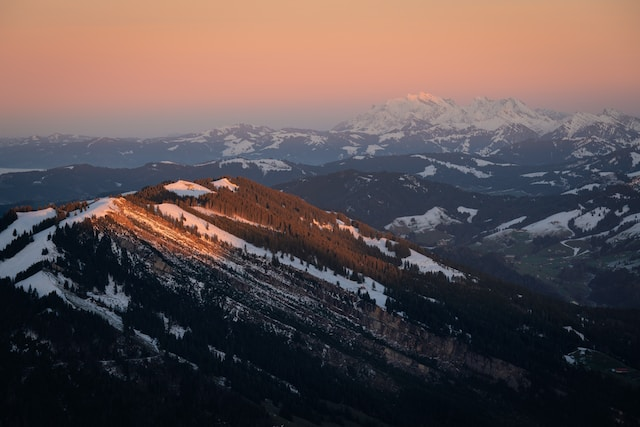
\includegraphics[scale=0.5]{1.jpg}

\begin{center}
    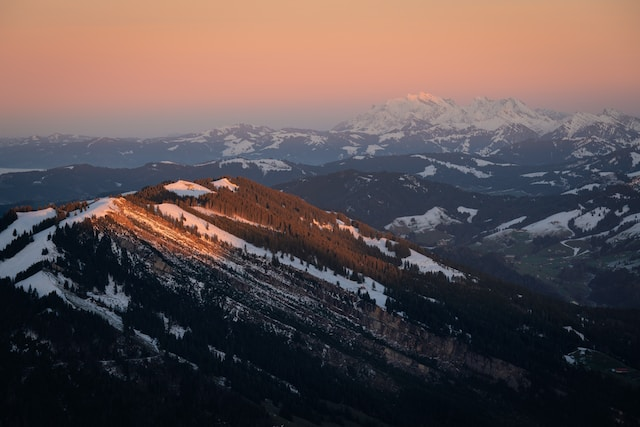
\includegraphics[width=3.5in]{1.jpg}
\end{center}

\begin{figure}[H]
    \centering
    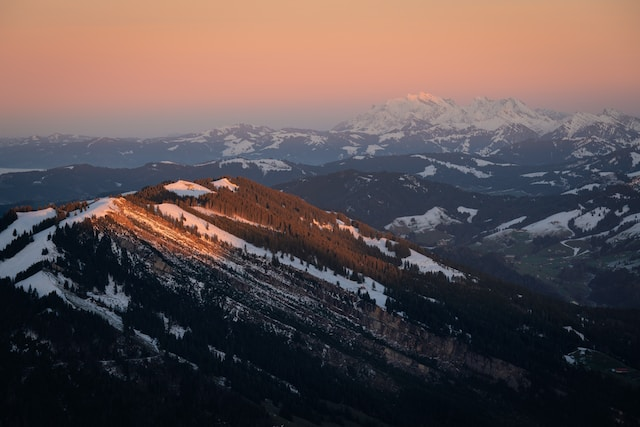
\includegraphics[width=3.5in]{1.jpg}
    \caption{This is a caption.}
\end{figure}

\end{document}